<<<<<<< generalinfo.tex
\documentclass{article}
\usepackage{url}
\usepackage{a4wide}
\usepackage{graphicx}
\usepackage[normal]{papersize}

\usepackage{fancyhdr}

%%[CL,CDSF,a4paper,Large,12pt]{OUCLdocument}

%\font\crestfont=newcrest scaled\magstep3
%\def\crest{{\crestfont \char1}}
\def\crest{\includegraphics[width=2cm]{crest}}

\def\covertiny{\fontsize{6}{7}\normalfont\selectfont}
\def\coverscriptsize{\fontsize{8}{9.5}\normalfont\selectfont}
\def\coverfootnotesize{\fontsize{9}{11}\normalfont\selectfont}
\def\coversmall{\fontsize{10}{12}\normalfont\selectfont}
\def\covernormalsize{\fontsize{11}{13.6}\normalfont\selectfont}
\def\coverlarge{\fontsize{12}{14}\normalfont\selectfont}
\def\coverLarge{\fontsize{14}{18}\normalfont\selectfont}
\def\coverLARGE{\fontsize{17}{22}\normalfont\selectfont}
\def\coverhuge{\fontsize{20}{25}\normalfont\selectfont}
\def\coverHuge{\fontsize{25}{30}\normalfont\selectfont}

\def\mktitle#1#2#3#4{
\null \noindent \raisebox{0.5cm}[0pt][0pt] { \hskip-3cm
 \makebox[21cm]{
\parbox[t]{4cm}{ \crest }
\parbox[b]{10cm}{\centering {\coverLARGE \textbf{#1}}\\
\vskip .1in {\coverlarge #2} \vskip 10pt }
\hfil
\parbox[b]{4cm}{\raggedleft \covernormalsize #4 }
} } }

%\newdimen\hdrtopskip
%\newdimen\hdrfootskip
%\newdimen\hdrwidth
%\newdimen\ftwidth
%\def\hdrsf{cmss}
%\def\hdrHugesize{\fontsize{25}{29}}
%\def\hdrsmall{\fontsize{5}{6}\fontfamily{\hdrsf}\selectfont}
%\def\hdrnormal{\fontsize{7}{8}\fontfamily{\hdrsf}\selectfont}
%\def\hdrLarge{\fontsize{12}{16}\fontfamily{\hdrsf}\selectfont}
%\def\hdrhuge{\fontsize{17}{21}\fontfamily{\hdrsf}\selectfont}
%\def\hdrHuge{\hdrHugesize\fontfamily{\hdrsf}\selectfont}
%\def\hdrline{1.8pt }
%\def\hdrmargin{15mm }
%\def\hdrtop{10mm }
%\def\hdrcresttop{3mm }
%\def\hdrbot{10mm }
%\def\hdrOUCL{Oxford University Computing Laboratory}
%\def\hdraddr{Wolfson Building, Parks Road, Oxford OX1 3QD}
%\def\fax{73839}
%\def\enquiries{73838}
%\def\www{http://www.comlab.ox.ac.uk/}
%\def\ukprefix{\@pls44 }
%\def\telprefix{\ukprefix1865 2}
%\def\emailsuffix{@comlab.ox.ac.uk}
%\def\profnames{     \slshape Director&Professor Bill Roscoe&73859&Email:~~Bill.Roscoe\crcr}
%\def\groupname{Programming Research Group}
%\def\OUCLheader{%
%   \hskip-\themargin
%   \hskip-1in \hbox to\paperwidth{%
%      \hskip\hdrmargin
%      \vbox to 0pt{
%         \vskip\hdrtopskip\vskip\hdrcresttop
%         \hbox to \hdrwidth{\hdrHuge \hdrOUCL}
%         \ifx\groupname\empty
%         \else\hdrhuge\hbox to \hdrwidth{\hfil\groupname\hfil}
%         \fi
%         \hdrLarge\hbox to \hdrwidth{\hfil\hdraddr\hfil}
%         \hdrnormal\vskip-.3\baselineskip
%         \null\hrule height\hdrline\null
%         \ialign to \hdrwidth{\tabskip=0pt plus1fil
%            {##\/}:\hfil&##\hfil&\telprefix##\hfil&\hfil##\emailsuffix
%            \tabskip=0pt\crcr
%            \profnames\crcr
%         }
%         \vss
%      }%
%      \hfil
%      \vbox to 0pt{\vskip\hdrtopskip\hbox{\crest}\vss}%
%      \hskip\hdrmargin
%   }\hss
%}


=======
\documentclass{article}
\usepackage{cramp2e}
\usepackage{url}
\usepackage{times}
\usepackage{graphicx,shadowbox}
%\usepackage[polish]{babel}
%\usepackage[normal]{papersize}
\fboxsep  = 5pt % making the shadow box smaller (default = 10pt)
\shadowwidth = 2pt % making the shadow smaller (default = 4pt)

\usepackage{fancyhdr}

%%[CL,CDSF,a4paper,Large,12pt]{OUCLdocument}

%\font\crestfont=newcrest scaled\magstep3
%\def\crest{{\crestfont \char1}}
\def\crest{\includegraphics[width=2.25cm]{newcrest}}

\def\covertiny{\fontsize{6}{7}\normalfont\selectfont}
\def\coverscriptsize{\fontsize{8}{9.5}\normalfont\selectfont}
\def\coverfootnotesize{\fontsize{9}{11}\normalfont\selectfont}
\def\coversmall{\fontsize{10}{12}\normalfont\selectfont}
\def\covernormalsize{\fontsize{11}{13.6}\normalfont\selectfont}
\def\coverlarge{\fontsize{12}{14}\normalfont\selectfont}
\def\coverLarge{\fontsize{14}{18}\normalfont\selectfont}
\def\coverLARGE{\fontsize{17}{22}\normalfont\selectfont}
\def\coverhuge{\fontsize{20}{25}\normalfont\selectfont}
\def\coverHuge{\fontsize{25}{30}\normalfont\selectfont}

\def\mktitle#1#2#3#4#5#6#7#8{
\null \noindent \raisebox{-1cm}[0pt][0pt] { 
\hskip-3cm
\makebox[21cm]{
\raisebox{-0.5cm}{\parbox[t]{5.75cm}{\hskip 1.85cm  \crest  }}
\raisebox{-0.5in}{\parbox[b]{8cm}{\centering {\coverLARGE \textbf{#1}} \\
\vskip .1in {\coverlarge #2} \vskip 10pt }}
\hfil
\raisebox{-0.2cm}{\parbox[b]{4.25cm}{\raggedleft \covernormalsize #4 \\ #5 \\ #6 \\ #7 \\ #8 }}
} } }

%\newdimen\hdrtopskip
%\newdimen\hdrfootskip
%\newdimen\hdrwidth
%\newdimen\ftwidth
%\def\hdrsf{cmss}
%\def\hdrHugesize{\fontsize{25}{29}}
%\def\hdrsmall{\fontsize{5}{6}\fontfamily{\hdrsf}\selectfont}
%\def\hdrnormal{\fontsize{7}{8}\fontfamily{\hdrsf}\selectfont}
%\def\hdrLarge{\fontsize{12}{16}\fontfamily{\hdrsf}\selectfont}
%\def\hdrhuge{\fontsize{17}{21}\fontfamily{\hdrsf}\selectfont}
%\def\hdrHuge{\hdrHugesize\fontfamily{\hdrsf}\selectfont}
%\def\hdrline{1.8pt }
%\def\hdrmargin{15mm }
%\def\hdrtop{10mm }
%\def\hdrcresttop{3mm }
%\def\hdrbot{10mm }
%\def\hdrOUCL{Oxford University Computing Laboratory}
%\def\hdraddr{Wolfson Building, Parks Road, Oxford OX1 3QD}
%\def\fax{73839}
%\def\enquiries{73838}
%\def\www{http://www.comlab.ox.ac.uk/}
%\def\ukprefix{\@pls44 }
%\def\telprefix{\ukprefix1865 2}
%\def\emailsuffix{@comlab.ox.ac.uk}
%\def\profnames{     \slshape Director&Professor Bill Roscoe&73859&Email:~~Bill.Roscoe\crcr}
%\def\groupname{Programming Research Group}
%\def\OUCLheader{%
%   \hskip-\themargin
%   \hskip-1in \hbox to\paperwidth{%
%      \hskip\hdrmargin
%      \vbox to 0pt{
%         \vskip\hdrtopskip\vskip\hdrcresttop
%         \hbox to \hdrwidth{\hdrHuge \hdrOUCL}
%         \ifx\groupname\empty
%         \else\hdrhuge\hbox to \hdrwidth{\hfil\groupname\hfil}
%         \fi
%         \hdrLarge\hbox to \hdrwidth{\hfil\hdraddr\hfil}
%         \hdrnormal\vskip-.3\baselineskip
%         \null\hrule height\hdrline\null
%         \ialign to \hdrwidth{\tabskip=0pt plus1fil
%            {##\/}:\hfil&##\hfil&\telprefix##\hfil&\hfil##\emailsuffix
%            \tabskip=0pt\crcr
%            \profnames\crcr
%         }
%         \vss
%      }%
%      \hfil
%      \vbox to 0pt{\vskip\hdrtopskip\hbox{\crest}\vss}%
%      \hskip\hdrmargin
%   }\hss
%}


>>>>>>> 1.28

% Traditional Oxford crest COMMENT OUT UNTIL I GET THE IMAGES
%\font\crestfont=oxcrest40 scaled\magstep3
%\def\crest{{\crestfont \char1}}
%For this to work on the Comlab network replace the first line above with
%\font\crestfont=crest scaled\magstep3

%New Oxford Belt crest
% \font\beltcrestfont=oxbeltcrest
% \def\beltcrest{{\beltcrestfont \char0}}
%For this to work on the Comlab network replace the first line above with
%\font\beltcrestfont=newcrest

%\title{Computer Science Logic 2005}
%\author{General Information}


<<<<<<< generalinfo.tex
\begin{document}
%\OUCLheader
%\vskip 5cm
=======
>>>>>>> 1.28

<<<<<<< generalinfo.tex
\mktitle{Computer Science Logic 2005}{General
Information}{1.0}{Oxford University \\ Computing Laboratory \\ \ \\}
=======
%\def\street#1{\vskip 0.1cm \noindent {\textbf{\underline{#1}}}}
\newenvironment{streetenum}{\begin{enumerate}}{\end{enumerate}}
\def\street#1{\item #1 }

\newcommand\privatenote[1]{\noindent\makebox[\textwidth][l]{\hrulefill}
\noindent\textbf{\small Note.}~~{\small #1}\\
\makebox[\textwidth][l]{\hrulefill}}
>>>>>>> 1.28

<<<<<<< generalinfo.tex
\section*{Location}
The conference will now be held in the Denis Wilkinson Building
(number 38 on the map below), Physics Department, and the terminal
room will be the room directly opposite the Dennis Sciama Lecture
Theatre.
\\
=======
        \newcommand\textbfit[1]{{\bf\em #1}\index{#1}}
>>>>>>> 1.28

<<<<<<< generalinfo.tex
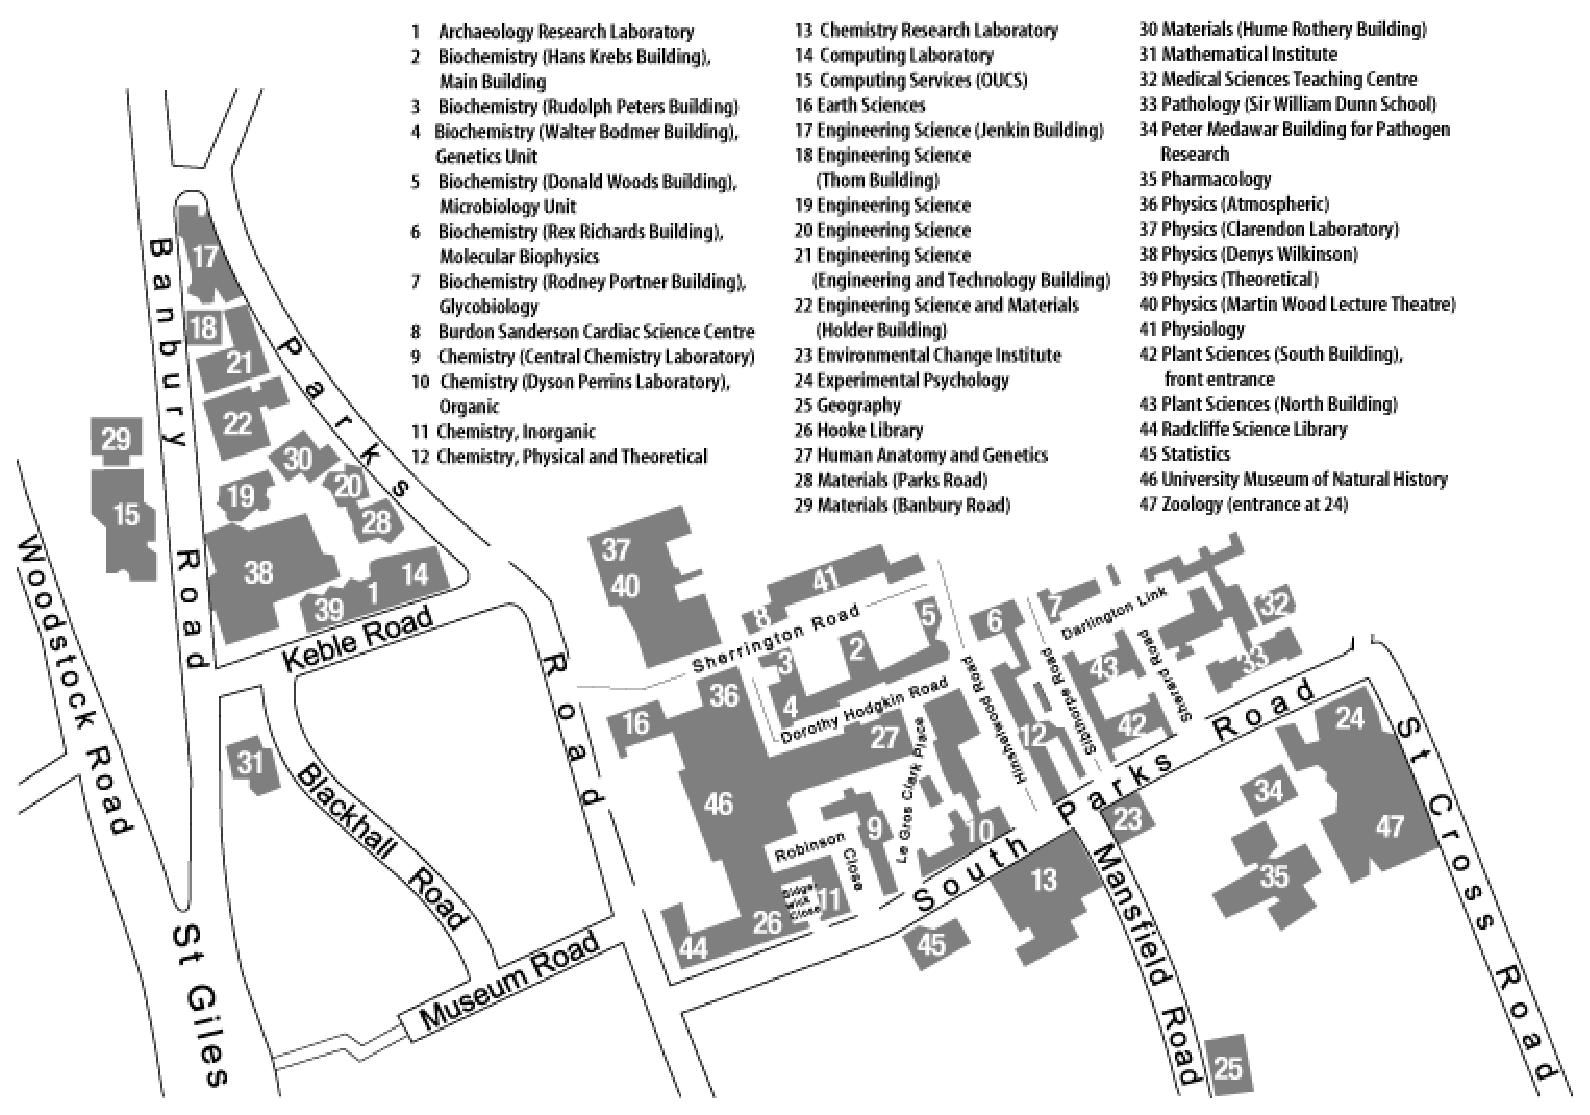
\includegraphics[width=15cm]{sciencearea}
=======
\begin{document}
%\OUCLheader
%\vskip 5cm
>>>>>>> 1.28

<<<<<<< generalinfo.tex
=======
%\vspace{1cm}
>>>>>>> 1.28

<<<<<<< generalinfo.tex
\section*{Internet Access}
6 PC/workstations are provided for participants to check their email
and access the Internet.
=======
%\mktitle{\Large Computer Science Logic 2005\\[2mm]22 - 25 August,
%  Oxford, UK}{\large Programme and General Information}{0}{Computing Laboratory}{Oxford
%  University }{Parks Road}{Oxford}{OX1 3QD}

\mktitle{}{}{1.0}{Computing Laboratory}{Oxford University}{Parks Road}{Oxford}{OX1 3QD}

\vspace{2cm}

\begin{center}
\LARGE {\bf Computer Science Logic 2005}\\[2mm]
\Large 14th Annual Conference of the European Association of Computer
Science Logic\\
22 - 25 August 2005, Oxford\\[3mm]

\huge \textbf{Conference Programme and General Information}\\

%\bigskip \shbox{\normalsize Draft of 16 August}
\end{center}

\bigskip

\begin{center}
\textbf{\large Programme Committee}

\bigskip

\begin{tabular}{ll}
Albert Atserias (Universitat Polit\`cnica de Catalunya)
& Aart Middeldorp (U.~of Innsbruck, Austria) \\
David Basin (ETH Z\"{u}rich)
& Dale Miller (INRIA / Ecole Polytechnique)\\
Martin Escardo (U.~of Birmingham)
& Damian Niwi\'nski (U.~of Warsaw)\\
Zoltan Esik (U.~of Szeged/Tarragona)
& Peter O'Hearn (Queen Mary, U.~of London)\\
Martin Grohe (Humboldt-Universit\"{a}t Berlin)
& Luke Ong (U.~of Oxford, Chair)\\
Ryu Hasegawa (U.~of Tokyo)
& Alexander Rabinovich (U.~of Tel Aviv)\\
Martin Hofmann (Ludwig-Maximilians-Universit\"{a}t M\"{u}nchen)
& Thomas Schwentick (Philipps-Universit\"{a}t Marburg)\\
Ulrich Kohlenbach (Darmstadt U.~of Technology)
& Alex Simpson (U.~of Edinburgh)\\
Orna Kupferman (Hebrew U.~of Jerusalem)
& Nicolai Vorobjov (U.~of Bath)\\
Paul-Andre Mellies (CNRS / Universit\'e Paris 7)
& Andrei Voronkov (U.~of Manchester)
\end{tabular}
\end{center}

%\newpage
%\tableofcontents
%\newpage

\section{The Conference at a Glance}
\textbf{CSL 2005} is the 14th annual conference of the European
Association for Computer Science Logic (EACSL). The conference series
started as a programme of International Workshops on Computer Science
Logic, and then in its 6th meeting became the Annual Conference of
the EACSL. The conference is intended for computer scientists whose
work involves logic, and for logicians working on topics relevant to
computer science.

\begin{tabular}{ll}
\textbf{Spectrum Workshop begins} & 09:45 Sunday 21 August, Fitzjames
Room 1, Merton College\\
\textbf{Reception and registration} & 18:00-20:00 Sunday 21 August, Savile
Room, Merton College\\
\textbf{Conference begins} & 09:00 Monday 22 August, Dennis Sciama
Lecture Theatre\\
\textbf{Meeting of EACSL} & 19:00 Monday 22 August, Fitzjames Room 1,
Merton College\\
\textbf{Excursion to Bletchley Park} & Afternoon of Tuesday 23 August;
coaches leave at 13:15\\
\textbf{2005 Ackermann Award Presentation} & 16:30 - 17:45 Wednesday
24 August, Dennis Sciama
Lecture Theatre\\
\textbf{Guided Tour of Merton College} & 17:00-17:45 Sunday 21 August
and
18:30-19:15 Wednesday 24 August\\
\textbf{Banquet} & 19:30 Wednesday 24 August, Merton College\\
\textbf{Conference ends} & 18:00 Thursday 25 August\\
\end{tabular}

\section{Getting to Oxford}

\textbf{Arriving by Air}.  There is a very convenient bus service from
\textbf{London Heathrow} to Oxford, \textbfit{the airline}, that runs
every 20 minutes. A return fare is \pounds 18. The journey takes 70 -
90 minutes. The bus may be boarded from Bay 14, Central Bus Station if
you arrive at Terminals 1, 2 and 3; or at Bay 15 if you arrive at
Terminal 4. For further information on the service (timetables, etc.)
see the Oxford Bus Company website
\url{http://www.oxfordbus.co.uk/}. Tickets may be bought on the bus.
If you arrive at \textbf{London Gatwick}, you can board \emph{the
airline} from Gatwick North Terminal Bay 4. The service runs every
hour. A return fare is \pounds 24. The journey takes roughly 120
minutes.

The \emph{airline} bus will terminate at the Gloucester Green Bus
Station in Oxford city centre; you will be able to catch a taxi there.
If you are staying at Merton College, you may wish to get off at the
Queen's Lane (which is off High Street) stop -- Merton College is
roughly 200 metres away.

\medskip

If you arrive at the \textbf{London City Airport}, take the Airport
Shuttlebus to Liverpool Street Underground Station, and then take the
Underground train to Paddington Station. You will be able to catch a
train to Oxford from the Paddington Rail Station. The train journey
will take approximately an hour.

\medskip

\noindent\textbf{Arriving by Train}. If travelling by train, you will arrive
at the Oxford Rail Station.  Merton Colleges and most hotels are a
long walk from the Station, and you will probably want to proceed by
taxi. Taxis arrive continuously, and you shouldn't have to wait long.

\section{The Conference Location: Denys Wilkinson Building}

The Conference will be held in the \textbf{Dennis Sciama Lecture
Theatre}, \textbf{Denys Wilkinson Building}, which is part of the
Department of Physics (number 38 on the map below).  Access to the
Building is from the Banbury Road end of Keble Road, via the concrete
stairs (just next to a bicycle shed).
>>>>>>> 1.28

<<<<<<< generalinfo.tex
\section*{Accomodation}
=======
\noindent \textbf{Tea and coffee breaks} will be at the 5th floor
foyer area, Denys Wilkinson Building.
>>>>>>> 1.28

<<<<<<< generalinfo.tex
Merton college...
=======
\medskip
>>>>>>> 1.28

<<<<<<< generalinfo.tex
=======
\begin{center}
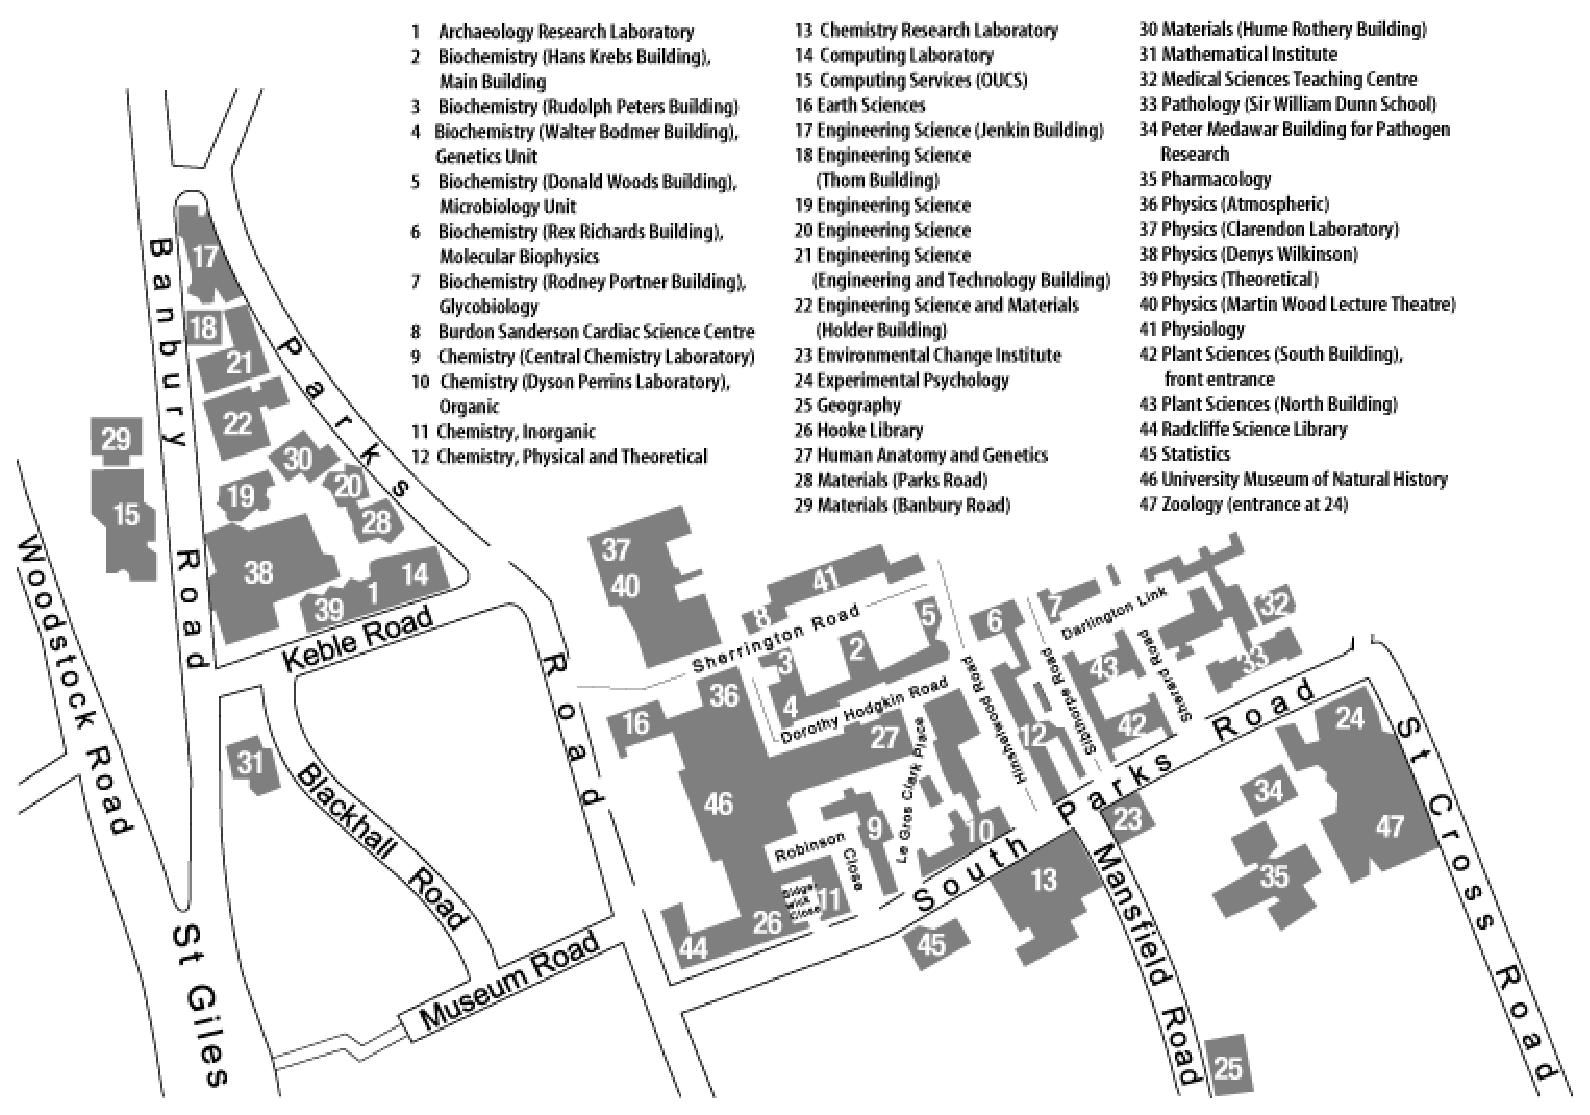
\includegraphics[width=15cm]{sciencearea}
\end{center}
>>>>>>> 1.28

<<<<<<< generalinfo.tex
\section*{Excursion}
=======
>>>>>>> 1.28

<<<<<<< generalinfo.tex
On Tuesday 23rd August we have arranged a coach trip Bletchley Park. \\
\\
\url{http://www.bletchleypark.org.uk/}

\begin{quote}
During World War II the German armed forces top secret codes were broken at
Bletchley Park, providing the allies with vital information towards their war effort.
Situated 50 miles North-West of London, the site played host to a diverse group of
code breakers, including Alan Turing and Dilly Knox. Among the ciphers that were
broken were Enigma and Lorenz.
\end{quote}

The coach will be leaving from outside the Wolfson Building, Parks Road (map reference E2) at 1330.  We will be leaving Bletchley Park at 1730 and expect to arrive back at the Wolfson Building around 1815.


\section*{Banquet}

There's a banquet...

\section*{Meals}

Meals are not provided.  Below is a list of eateries in Oxford.
Map references apply to both \textit{Oxford by Day} and \textit{Oxford by Night}, although some places may be marked on one but not the other.  Some places are not shown on either.
=======
\subsubsection*{Please Note:} 
\begin{itemize}
\item \textbfit{Do wear your badges at all times}. We have been told
that from Monday 22 August noon onwards, no participant will be
allowed into the Denys Wilkinson Building without their participant
badge. 

\item \textbfit{No eating or drinking is permitted in the Dennis Sciama Lecture
Theatre.}

\item \textbfit{We need to vacate the Lecture Theatre by 6pm on
  Monday, Wednesday and Thursday} - please cooperate.
\end{itemize}

\subsubsection*{From Merton College to the Denys Wilkinson Building}
\textbf{Merton College} and the \textbf{Denys Wilkinson Building} are
marked out in the following map. There is a straightforward route from
the College to the DW Building (indicated in green): Magpie Lane
(which is off the cobblestoned Merton Street), Catte Street, Parks
Road, and then Keble Road. The journey takes about 15 minute on foot.

\medskip

\begin{center}
\includegraphics[width=15cm]{approach}
\end{center}

\section{Information for Speakers}
The Dennis Sciama Lecture Theatre has a \textbf{blackboard}, an
\textbf{overhead slide projector} and a \textbf{data projector}.  If
you use computer-generated slides, you should liaise with the
audio-visual technician during the coffee/tea breaks or early in the
day (08:45-09:00) to load up your presentations well before your talk.

Speakers are requested to \textbf{end their talk 5 mins before} the
alloted time, so as to leave some time for questions.

\section{Reception and Registration}
The first pre-conference event is a \textbf{guided tour of Merton
College}, 17:00-17:45 Sunday 21 August. The assembly point is just
outside the Porter's Lodge.

There will be a drinks reception 18:00-20:00 Sunday 21 August, in the
\textbf{Savile Room, Merton College} at (the cobblestoned) Merton
Street; some finger food will also be served. You will be able to
register for the conference during the reception. 

For those who miss the reception, there will be another opportunity to
register at 08:30 Monday 22 August, just before the start of the
conference at the \textbf{Registration Desk (Tel: +44 1865 273434)},
which is in the foyer of the Dennis Sciama Lecture Theatre.


\section{Email and Internet Access}
The \textbf{Internet Room} is directly opposite the Dennis
Sciama Lecture Theatre, in the Denys Wilkinson Building.  A number of
workstations, preset to webdemo mode, are provided for participants to
check their email (by \textsc{ssh}) and access the Internet.

\noindent\textbf{Wireless network}.  There is a wireless network
covering the Dennis Sciama Lecture Theatre, the Internet Room, and the
General Common Room in the Dennis Wilkinson Building.  If you have
given us the MAC address of your laptop, you should be able to gain
access by setting the following parameters:

\begin{tabular}{ll}
\textbf{Service Set Identifier (SSID)} & \texttt{Physics\_M}\\
\textbf{WEP 128-bit encryption key} & \texttt{f672c67945b4478ff9145571df}
\end{tabular}

\noindent When in the Denys Wilkinson Building, some laptops may pick
up the SSID automatically. Unfortunately Merton College is unable to
provide any IT facilities for conference residents.

\section{Merton College}

Merton College was founded in 1264. It is one of three ancient Oxford
colleges founded in the thirteenth century. The College buildings, set
in extensive gardens and grounds, are of exceptional historical and
aesthetic interest. The Library is probably the oldest surviving
working library in the United Kingdom, and the Hall, Chapel, Lodge and
Mob Quadrangle also date from the College's early years.

The College's founder was Walter de Merton, Lord Chancellor of England
and Bishop of Rochester. Walter's conception of a self-governing
community of scholars, with its own statutes and endowment, residing
in buildings laid out in staircases and quadrangles, created a model
and precedent for Oxford and Cambridge colleges founded in the
succeeding centuries.

Merton College is one of many colleges that, together with
departments, faculties, laboratories, libraries and other academic
institutions, comprise the University of Oxford.  The relationship
between the Oxford colleges and the University has evolved throughout
the centuries. The colleges are self-governing institutions that
provide academic, domestic and social facilities to their student
members. Teaching provision for most undergraduate degree courses at
Oxford is concentrated in the colleges, but examinations are
administered by the University, which has sole power to confer
degrees.

Merton College is administered by a Governing Body consisting of the
Warden and Fellows. The Warden is the Head of College. The Fellowship
includes teaching Fellows, or Tutors, who are responsible for tuition
and pastoral care of undergraduates. Most Tutors also have University
duties. Other Fellows include Professorial Fellows (who also hold
University posts), Research Fellows and College Officers, such as the
Senior Tutor, Librarian, Chaplain and Bursar.

%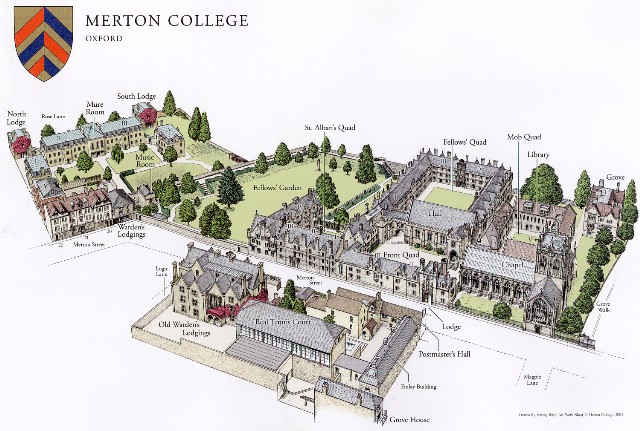
\includegraphics[width=14cm]{mertonLargeWebview}

\subsection*{Merton College Accommodations}

\noindent\textbf{Arrival}. If you have reserved Merton College
accommodation, please call at the Porter's Lodge directly on
arrival. The Porter will explain how to get to your room, and give you
your room key, and a late gate key, which can be used to enter and
leave the College when the Lodge gate is closed between 22:30 and
07:00. Please retain your keys for the duration of your stay with
us. \textbf{Breakfast} will be served at 07:45 in the Hall.

\medskip

\noindent\textbf{Departure}. You are requested to vacate your room by
10:00 on the last day of the conference. Please remember to return
your keys to the College Lodge.

\medskip

\noindent\textbf{Contact Information}. If you need information about
the College facilities, please contact the Conference Manager, Mrs Kim
Cameron (tel.~(2)76363) during office hours 09:30 - 17:30 Monday to
Friday, or the duty porter (tel.~(2)76310) at any time. Please note the
Porter should not be contacted between 23:00 and 07:00 except in
emergency.

\medskip

\noindent\textbf{Guided Tour of the College}. There will be a guided tour of
the College, including a visit to the Old Library (the oldest library
in Britain in continuous use), at the following times:

\begin{tabular}{l}
17:00-17:45 Sunday 21 August\\ 18:30-19:15 Wednesday 24 August
\end{tabular}

\noindent Please assemble just outside the Porter's Lodge. Each tour
will be limited to a maximum of 20 people, on a first come first serve
basis. 

\medskip
 
For further information, see the \emph{Information for
Delegates}. There is a map of the College in the \emph{Guide to Merton
College}.

\section{Excursion to Bletchley Park}

On Tuesday 23rd August we have arranged a trip to \textbf{Bletchley
Park}. During World War II the German armed forces top secret codes
were broken at Bletchley Park, providing the allies with vital
information towards their war effort.  Situated 50 miles North-West of
London, the site played host to a diverse group of code breakers,
including Alan Turing and Dilly Knox. Among the ciphers that were
broken were Enigma and Lorenz. For further details, see
\url{http://www.bletchleypark.org.uk/}.  

We will travel to Bletchley Park by coach. \textbfit{The coaches will
leave from the junction of Keble Road and Parks Road at 13:15, Tuesday
23 August}. We will leave Bletchley Park at 17:30 and expect to arrive
back at Oxford around 18:15, traffic permitting.

\section{Banquet}
For those who missed the Sunday tour, there will be another
\textbf{guided tour of Merton College}, 18:30-19:15 Wednesday 24
August, just before the banquet. Please assemble just outside the
Porter's Lodge. 

The conference banquet will be held in the Hall of the College.

\medskip

\begin{center}
\mbox{
\begin{shadowbox}[12cm]
\begin{center}
\medskip
{\textbfit{\Large CSL2005 Banquet}}\\
\medskip
\emph{19:30 Wednesday 24th August 2005, Merton College, Oxford}\\

\bigskip

\begin{tabular}{c}
Hot and sour prawn soup\\
        Roast beef with oyster sauce\\
        Ginger ice-cream\\
        Cheese platter\\
\\
Coffee / Tea\\
\\
\emph{St.~Martin de la Garrigue '99}\\
\end{tabular}
\end{center}
\end{shadowbox}}
\end{center}

\section{Restaurants and Other Eateries}

Meals are not provided.  Below is a list of eateries in Oxford.  Map
references apply to both \textit{Oxford by Day} and \textit{Oxford by
Night}, although some outlets may be marked on one but not the other.
Others are not shown on either.
>>>>>>> 1.28

\emph{Daily Info} has quite a good restaurant guide at
\url{http://www.dailyinfo.co.uk/food/restaurants.html}

\subsection*{Lunches}

Since there isn't much time for a proper, leisurely lunch, if you wish
to have a sandwich or baguette, you can get a good selection from
Taylors Delicatessen or Felson's Sandwich Bar, which are at opposite
ends of Little Clarendon Street, about 5 mins walk from the Denys
Wilkinson Building. Weather permitting, a good place to enjoy your
baguette is in the University Park.

\medskip

The following is a list of places where you can get lunch. Also see
\textit{pubs and bars}.

\begin{streetenum}
\street{Little Clarendon/Woodstock Road} Map reference C2-D2.
\begin{description}
\item[Taylors Delicatessen] St Giles/Little Clarendon Street. Delicatessen and Sandwich
Shop.
\item[Felson's Sandwich Bar] End of Little Clarendon Street.

\item[George and Davis Ice Cream Shop (G \& D's)] Serves pizza, bagels, ice cream and more.  Open until midnight.
\item[Mortons] Baguettes for \pounds 2.50 and panini for \pounds 3.
\item[Porters] Lunch course with soft drink for \pounds 5.
\item[Maison Blanc] French Patisserie. Sandwiches approx. \pounds 4. 

\item[Browns] 5-11 Woodstock Road. Sandwiches \pounds 6-8.
\item[Wok\&Roll] 4-6 Woodstock Road. Takeaway for \pounds 4.50.
\end{description}

\street{Holywell street} Map reference F4-G4.
\begin{description}
\item[Edamam\'e] 15 Holywell Street. Japanese; tiny, clean, light and
  fast.

\item[The Alternative Tuck Shop]

\item[Holywell's Bar \& Brasserie] 38 Holywell St.

\end{description}

\street{George street} Map reference D5.
\begin{description}
\item[Caf� Opium] Corner of George Street. Set menu \pounds 12-20. Dishes at approx. \pounds 5.

\item[Caff� Uno] Lunch from \pounds 4.95. Pizza \pounds 6-9.

\item[Pizza Hut] George Street south side.

\item[Zizzi] 59 George Street. Pizza from \pounds 5.20 to \pounds
7.50. Pizza to go at \pounds 5.

\item[Yates$^s$] ``Great plates'' for \pounds 7.
\item[Caff� Uno] Lunch from \pounds 5. Pizza \pounds 6-9.

\item[Le Parisien] Sandwich \pounds 1.80-2.
\item[La Croissanterie] ``French'' sandwiches \pounds 1.70-3. Panini
\pounds  2.60.
\end{description}

\street{Market Square}

Market Square lies behind the Odeon Cinema on George Street and Gloucester Green Coach Station.  Map reference D5.

\begin{description}

\item[Noodle Bar] Cheap noodles.  \pounds 4-5.

\item[Cleo's Cafe] Sweet and savoury crepes.  Free chocolate crepe with every savoury crepe.  \pounds 4.50.

\item[Harveys] Made to order hot sandwiches.  \pounds 2-3.

\item[Cafe Piazza] Sandwiches, bagels, baguettes and ciabattas for \pounds 3-4.


\end{description}


\street{Cornmarket Street}

\begin{description}

\item[Sainsbury's Local] On Magdelen Street. Map reference E4.  Sells
pre-packaged sandwiches for \pounds 1.50-3.

\item[Fast Food] The standard fast food places are all represented on
Cornmarket Street (KFC, Burger King, McDonalds).  Burger King and KFC
are on the George Street side, whilst McDonalds is towards the High
Street.  Meals (burger, fries, drink) are roughly \pounds 4.

\item[St Michael's Street] St Michaels Street is just off Cornmarket
Street.  There are two lunch places.  The Nosebag serves salads, baked
potatoes, soup, etc. for \pounds 4-5.  Meltz serves sandwiches, salads
and pasta for \pounds 5-7.

\item[Ship Street] Ship street is opposite St Michael's Street.  The
News Cafe sells salads, pasta, bagels for \pounds 5-8.50.  Heroes sell
sandwiches made to order for \pounds 3-4 (takeaway, plus 20\% eat-in).

\item[West Cornwall Pasty] Near the High Street.  Sells pre-made
cornish pasties for \pounds 2.50.

\item[Golden Gate Covered Market] Entrance near West Cornwall Pasty.
There are many cafes within the market, plus Pizza Express --- which
sells pizzas for \pounds 6-8 and salads and pasta for \pounds 7-8 ---
and Cafe Puccino --- which sells salads, paninis, ciabattas,
baguettes, baked potatoes and tapas for roughly \pounds 6.

\item[Pret] Near the High Street.  Sells packaged sandwiches (more
interesting than Sainsbury's) for \pounds 2-3.

\end{description}

\end{streetenum}



\subsection*{Restaurants}

Also see \textit{pubs and bars}.

\begin{streetenum}

\street{High Street / St. Clements}

\begin{description}

\item[Pizza Express] Map reference E5.  Sells pizzas, pasta and salads for \pounds 6-8.  Not as cheap and cheerful as Pizza Hut.

\item[Pizza Hut] Opposite The Chequers.  Map reference E6.  Pizzas
\pounds 5.50 for an individual.  On Tuesdays: eat as much as you like
for \pounds 7 (includes drink).

\item[Fishers] Map reference J6.  Sells seafood.  Main courses \pounds 12-15.

\item[Pink Giraffe] Map reference J6.  Chinese restaurant.  \pounds
8-9 for a meal.

\item[Thai Orchid] Map reference J6.  Thai restaurant.  \pounds 9-10
for a meal.

\item[Liaison] Map reference D6.  Chinese restaurant.  29 Castle Street.

\end{description}


\street{George Street} Map reference D5.

\begin{description}
\item[Peninsula] Chinese. 21 George Street. Set meal from \pounds 16-35.
\item[Noodle Bar] Noodles for \pounds 4-5.  Market Square, off George Street.
\item[ASK] 5 George Street. Pizza and pasta from \pounds 5 to \pounds 7.
\item[Caf\'e Opium] Chinese. 67-69 George Street.
\item[Tarbouch] Lebanese/Greek. 29 George Street.
\item[Bella Italia] Italian. 14/16 George Street. Pizza \pounds 5-8.
Dishes \pounds 10-14.
\item[Zizzi] Italian.
\end{description}

\street{Hollywell Street}
\begin{description}
\item[Edamame] Japanese.  15 Hollywell Street.  Map reference F4.
\end{description}


\street{Little Clarendon Street/Woodstock Road} Map reference C2-D2.

\begin{description}
\item[Pierre Victoire] 9 Little Clarendon Street. French. Dinner
from \pounds 9.90. Lunch from \pounds 5.90.
\item[La Plaza Tapas Bar] 10 Little Clarendon Street. Spanish. Lunch
from \pounds 5.95. Main course \pounds 9.
\item[Caf\'e Rouge] 11 Little Clarendon Street. French. Dinner from
\pounds 7.95.
\item[Porters] Restaurant and Bar.
\item[Browns] 5-11 Woodstock Road. Main course from \pounds 8 to
\pounds 16.
\item[Wok\&Roll] 4-6 Woodstock Road. Chinese restaurant and
takeaway. Set dinner from \pounds 15 to \pounds 36.
\end{description}

\end{streetenum}

\subsection*{Pubs and Bars}

Where mentioned, food is available.  Food is usually served until
about 1900 to 2030.  Standard pub food includes burgers, lasagne,
steak, sausage and mash, chicken tikka masala and fish and chips.
Pubs close at 2300, bars sometimes open later.

\begin{description}
\item[The Turf Tavern] Well-hidden, pokey and inexplicably popular.
Bath Place, off Holywell Street/Queen's Lane.  Map reference G4.
\item[The King's Arms] Corner of Parks Rd \& Holywell Street. Map
reference F4.
\item[Holywell's Bar \& Brasserie] 38 Holywell St. Map reference G4.
\item[Angels] Bar. Little Clarendon. Map reference C2.
\item[Duke of Cambridge] Pub. Little Clarendon. Map reference D2.
\item[The Grapes] 7 George Street. Map reference D5. Meal from \pounds 5
to \pounds 6.

\item[Cock and Camel] 24 George Street. Map reference D5.



\item[Lamb and Flag] Map reference D3.  Food \pounds 3.50-5.

\item[The Goose] By the Gloucester Arms.  Map reference D4.  Has a
large beer garden and the occasional barbeque.  Food roughly \pounds
5, with meal deals (with drink) starting from \pounds 3.

\item[Old Orleans] On George Street.  Map reference D5.  Mississippi
themed pub/restaurant, serves cajun and creole cooking.  Burgers
\pounds 7-10, main courses \pounds 9-13.

\item[Three Goats Heads] By the Oxford Union.  Map reference D5.  Has
an unusual selection of drinks.  Food \pounds 5-6.

\item[O'Neils] On George Street.  Map reference D5.  Chain Irish theme
pub.  Burgers \pounds 5, main courses \pounds 6-7.


\item[The Chequers] Map reference E6.  Has three pool tables and two
quiz machines.  Food \pounds 6.

\item[The Mitre] Map reference E5.  Food \pounds 8-12.

\item[The Pub Oxford] By the Cricketer's Arms.  Map reference I7.
Lots of games machines including a games console.  Food \pounds 5.

\item[Head of the River] Map reference E8.  Large beer garden on the
river.  Punting nearby.  Food \pounds 8-9.

\item[Freuds] Map reference C2.  A converted church with live music
and local art.  Serves calzone, bagels and ciabattas for \pounds 5-6.

\item[Baby] Map reference C2.  Mediterranean bar, serves cocktails.
Food \pounds 13.

\item[Copa] On George Street.  Map reference D5.  Serves a range of
continental beers.  Food \pounds 7-8.

\item[All Bar One] 124 High Street.  Wine bar aimed at over 21s.
Sharing platters for three \pounds 11.  Burgers, salads, steaks
\pounds 7-10.

\item[Quod] Map reference F5. Bar and grill.  Large sun terrace.  Food
\pounds 8-10.

\item[Thirst] Map reference B5.  Cheap cocktails, open late.



\end{description}

\section{Nighttime Entertainment}

Below is a description of some of the cinemas/theatre/etc. in Oxford.
Please check the websites for what's on information.  Map references
refer to \textit{Oxford by Night}.

For more information (including gigs and concerts), see the
\textit{What's On} section of \url{http://www.dailyinfo.co.uk/}.


\begin{description}

\item[Odeon Cinemas] Mainstream cinema.  Split between George Street
(map reference D5) and Magdalen Street (map reference D4).

\verb+http://www.odeon.co.uk/+ (go to ``Times and Booking (text
version)'' if Flash doesn't work.)

\item[Phoenix Picturehouse] Map reference B1.  More arthouse, but not
completely obscure.

\verb+http://www.picturehouses.co.uk/site/cinemas/Oxford/local.htm+

\item[Ultimate Picture Palace] Map reference J7.  No frills cinema
showing films from all over the world. Also fairly cheap.

\verb+http://www.ultimatepicturepalace.co.uk/+

\item[New Theatre] Map reference D5.  Lots of shows and musicals.

\verb+http://www.thisistheatre.com/regional/oxfordtheatre.html+


\item[Oxford Playhouse] Map reference D4.  As the name suggests, the
focus is on plays rather than shows.

\verb+http://www.oxfordplayhouse.com/+

\item[Jongleurs]  Map reference B5.  Stand-up comedy, unfortunately only on Thursdays, Fridays and Saturdays.

\verb+http://www.jongleurs.com/+


\end{description}


\section{Emergency and Other Information}

Prefix for Oxford phone numbers: + 44 1865. 

\noindent For more information about Oxford, visit the dailyinfo
website: \url{http://www.dailyinfo.co.uk/}.

\subsubsection*{Emergency Services}

The number for emergency services in the UK (Fire, Police, Ambulance)
is 999 or 112. The international standard emergency telephone number
for GSM mobile phone networks is 112.

\subsubsection*{Getting to London Heathrow or Gatwick}

You can catch the bus service, \textbfit{the airline}, from the
Gloucester Green Bus Station in the City Centre, or from a bus stop
along High Street (right next to Queen's Lane). 

\subsubsection*{Taxis}

\begin{description}
\item[Hackney Cabs] You can pick one up at a taxi rank at St.Giles, Gloucester Green
(tel: 770077), or the railway station. You can also hail Hackney
cabs in the street.


Fares: A minimum of \pounds 1.50, then about 90p per mile
    (Sample Fares:
    the city centre to any of the Park and Rides is about 3 miles and costs about \pounds 4,
      Heathrow - \pounds 55,
      Gatwick - \pounds 90,
      Central London - \pounds 75)


Hackney Cabs are licensed and limited in numbers by the city
council. However they are also reputed to have a generally better
local knowledge than drivers of hire cars.  They are made specifically
for their job and provide easier access for those with mobility
difficulties.


\item[Hire Cars] Hire cars (or minicabs) are not licensed individually
(rather on a per company basis) and are normally not specialised
vehicles.

They are not allowed to pick up passengers who hail them on the
street. You need to phone their HQ and they will send a vehicle for
you. They are often cheaper than a Hackney Cab.

Fares vary.

Contact: ABC Taxis: 770077 or 775577. RadioTaxis: 242424 or 249743.
001 Taxis: 240000. Royal Cars: 777333

\item[CCB Airport Cars] Tel: 876699. Run to and from Heathrow,
Gatwick, Luton and Birmingham.

\end{description}

\section{Sponsors}

The organisers would like to thank Merton College and the Computing
Laboratory for both financial support and much time from their staff.
Thanks are also due to the British Logic Colloquium for the gift of
student bursaries.

\vspace{1cm}

\begin{flushright}
\textbf{CSL05 Local Organizing Committee}\\
~\\
William Blum\\
Matthew Hague\\
Jolie de Miranda\\
Andrzej Murawski\\
Luke Ong\\
Sam Sanjabi\\
Nikolaos Tzevelekos\\
~\\
August 2005, Oxford\\
\end{flushright}


\newpage

\section{Conference Programme}
{\small
\subsection*{Sunday 21 August 2005}

\begin{tabular}{p{1cm}p{14.5cm}}
09:45 & \textbf{Spectrum Workshop begins}, Fitzjames Room 1, Merton College\\
17:00 & \textbf{Guided Tour of Merton College}, assemble just outside Porter's Lodge\\
18:00 & \textbf{Reception and Registration}, Savile Room, Merton College\\
\end{tabular}

\subsection*{Monday 22 August 2005}

\begin{tabular}{p{1cm}p{14.5cm}}
08:30 & \textbf{Registration}, foyer of Dennis Sciama Lecture Theatre,
Denys Wilkinson Building\\
%\\
& Chair: \emph{Luke Ong}\\
&	\textbfit{Semantics and Logics}\\
09:00 &	\emph{Ulrich Berger}. An Abstract Strong Normalization Theorem
(\emph{Invited Lecture})\\
10:00 &	\emph{Matthew Collinson, David Pym and Edmund Robinson}. On Bunched Polymorphism\\
%\\
\hline
10:30 & \multicolumn{1}{c}{\textbf{Coffee}}\\
\hline
%\\
& Chair: \emph{Ian Stark}\\
11:00 &	\emph{Tom Murphy, Robert Harper and Karl Crary}. Distributed Control Flow with Classical Modal Logic\\
11:30 &	\emph{Jiri Ad\'amek}. A Logic of Coequations\\
12:00 &	\emph{Shin-ya Katsumata}. A Semantic Formulation of $\top\top$-lifting and Logical Predicates for Computational Metalanguage\\
%\\
\hline
12:30 & \multicolumn{1}{c}{\bf Lunch}\\
\hline
%\\
& Chair: \emph{Ulrich Berger}\\
	& \textbfit{Type Theory and Lambda Calculus I}\\
14:00 & 	\emph{Paula Severi and Fer-Jan de Vries}. Order Structures on B\"ohm-like Models\\
14:30 & 	\emph{Colin Stirling}. Higher-order Matching and Games\\
%\\
	& \textbfit{Constructive Reasoning and Computational Mathematics I}\\
15:00 & 	\emph{Branimir Lambov}. Complexity and Intensionality in a
Type-1 Framework for Computable Analysis\\
%\\
\hline
15:30 & \multicolumn{1}{c}{\bf Tea}\\
\hline
%\\
& Chair: \emph{Luke Ong}\\
16:00 & 	\emph{Vasco Brattka and Matthias Schr\"oder}. Computing with Sequences, Weak Topologies and the Axiom of Choice\\
%\\
	& \textbfit{Linear Logic and Ludics I}\\
16:30 & 	\emph{Pierre-Louis Curien and Claudia Faggian}. L-nets, Strategies and Proof-nets\\
17:00 & 	\emph{Jean-Marc Andreoli, Gabriele Pulcini, and Paul Ruet}. Permutative Logic\\
17:30 & 	\emph{Kaustuv Chaudhuri and Frank Pfenning}. Focusing the Inverse Method for Linear Logic\\
%\\
\hline
	& \multicolumn{1}{c}{\textbf{Evening Event}}\\
\hline
%\\
19:00 & 	\textbf{EACSL Annual General Meeting}, Fitzjames Room 1, Merton College
\end{tabular}

\subsection*{Tuesday 23 August 2005}

\begin{tabular}{p{1cm}p{14.5cm}}
& Chair: \emph{Julian Bradfield}\\
09:00 & 	\emph{Matthias Baaz}. Proof Theory of Analogical Reasoning and
Juridical Logic (\emph{Invited Lecture})\\
%\\
	& \textbfit{Linear Logic and Ludics II}\\
10:00 & 	\emph{Esfandiar Haghverdi and Philip J. Scott}. Towards a Typed Geometry of Interaction\\
%\\
\hline
10:30 & \multicolumn{1}{c}{\textbf{Coffee}}\\
\hline 
%\\
& Chair: \emph{Bakhadyr Khoussainov}\\
	& \textbfit{Constraints}\\
11:00 & 	\emph{Hubie Chen and V\'ictor Dalmau}. From Pebble Games to Tractability: An Ambidextrous Consistency Algorithm for Quantified Constraint Satisfaction\\
11:30 & 	\emph{Ashish Tiwari}. An Algebraic Approach for the Unsatisfiability of Nonlinear Constraints\\
%\\
\hline
12:00 & 	\multicolumn{1}{c}{\bf Lunch}\\
\hline
%\\
13:15 & \textbf{Excursion to Bletchley Park}. The coaches will leave
from the junction of Keble Road and Parks Road at 13:15.
\end{tabular}

\subsection*{Wednesday 24 August 2005}

\begin{tabular}{p{1cm}p{14.5cm}}
& Chair: \emph{Janos Makowsky}\\
&	\textbfit{Finite Models, Decidability and Complexity}\\
09:00 & 	\emph{Maarten Marx}. XML Navigation and Tarski's Relation
Algebras
(\emph{Invited Lecture})\\
10:00 & 	\emph{Marcin Mostowski and Konrad Zdanowski}. Coprimality in Finite Models\\
%\\
\hline
10:30 & \multicolumn{1}{c}{\textbf{Coffee}}\\
\hline
%\\
& Chair: \emph{Etienne Grandjean}\\
11:00 & 	\emph{Michael Benedikt and Luc Segoufin}. Towards a Characterization of Order-Invariant Queries over Tame Structures\\
11:30 & 	\emph{Bakhadyr Khoussainov and Sasha Rubin}. Decidability of Term Algebras Extending Partial Algebras\\
12:00 & 	\emph{Emanuel Kiero\'nski}. Results on the Guarded Fragment with Equivalence or Transitive Relations\\
%\\
\hline
12:30 & 	\multicolumn{1}{c}{\bf Lunch}\\
\hline
%\\
& Chair: \emph{Neil Immerman}\\
14:00 & 	\emph{Bruno Courcelle and Christian Delhomm\'e}. The Modular Decomposition of Countable Graphs: Constructions in Monadic Second-Order Logic\\
14:30 & 	\emph{Balder ten Cate and Massiomo Franceschet}. On the Complexity of Hybrid Logics with Binders\\
15:00 & 	\emph{Julian Bradfield and Stephan Kreutzer}. The Complexity of Independence-Friendly Fixpoint Logic\\
%\\
\hline
15:30 & \multicolumn{1}{c}{\bf Tea}\\
\hline
%\\
& Chair: \emph{Bruno Courcelle}\\
16:00 & 	\emph{Antonina Kolokolova}. Closure properties of weak systems of bounded arithmetic\\
%\\
	& \textbf{2005 Ackermann Award Presentation}\\
16:30 & 	\emph{Johann Makowsky}, EACSL President and Jury Chair\\
16:45 &	\emph{Miko\l aj Boja\'nczyk}. Decidable Properties of Tree Languages\\
17:15 &	\emph{Konstantin Korovin}. Knuth-Bendix orders in automated deduction and term rewriting\\
& \emph{Nathan Segerlind}.
New Separations in Propositional Proof Complexity\\
%\\
\hline
	& \multicolumn{1}{c}{\textbf{Evening Event}}\\
\hline
%\\
18:30 & \textbf{Guided Tour of Merton College}, assemble just outside Porter's Lodge\\
19:30 & \textbf{Conference Banquet}, Merton College\\
\end{tabular}

\subsection*{Thursday 25 August 2005}
\begin{tabular}{p{1cm}p{14.5cm}}
& Chair: \emph{Damian Niwi\'nski}\\
	& \textbfit{Verification and Model Checking}\\
09:00 & \emph{Anatol Slissenko}. Verification in Predicate Logic with Time:
Algorithmic Questions (\emph{Invited Lecture}) \\
10:00 & 	\emph{Julian Bradfield, Jacques Duparc and Sandra Quickert}. Transfinite Extension of the Mu-Calculus\\
%\\
\hline
10:30 & \multicolumn{1}{c}{\textbf{Coffee}}\\
\hline
%\\
& Chair: \emph{Colin Stirling}\\
11:00 & 	\emph{Witold Charatonik, Lilia Georgieva and Patrick Maier}. Bounded Model Checking of Pointer Programs\\
11:30 & 	\emph{Carsten Lutz}. PDL with Intersection and Converse is Decidable\\
12:00 & 	\emph{Filip Murlak}. On Deciding Topological Classes of Deterministic Tree Languages\\
%\\
\hline
12:30 & 	\multicolumn{1}{c}{\bf Lunch}\\
\hline
%\\
%\\
& Chair: \emph{David Pym}\\
	& \textbfit{Type Theory and Lambda Calculus II}\\
14:00 & 	\emph{Fr\'ed\'eric Blanqui}. Decidability of Type-checking in the Calculus of Algebraic Constructions with Size Annotations\\
14:30 & 	\emph{Bruno Barras and Benjamin Gr\'egoire}. On the role of type decorations in the Calculus of Inductive Constructions\\
%\\
	& \textbfit{Constructive Reasoning and Computational Mathematics II}\\
15:00 & 	\emph{Mircea-Dan Hernest}. Light Functional Interpretation - an optimization of G\"odel's technique towards the extraction of (more) efficient programs from (classical) proofs\\
%\\
\hline
15:30 & \multicolumn{1}{c}{\bf Tea}\\
\hline
%\\
& Chair: \emph{Arnaud Durand}\\
16:00 & 	\emph{Michael Soltys}. Feasible Proofs of Matrix Properties with Csanky's Algorithm\\
%\\
	& \textbfit{Implicit Computational Complexity and Rewriting}\\
16:30 & 	\emph{Steven Perron}. A Propositional Proof System for Log Space\\
17:00 & 	\emph{Carsten Sch\"urmann and Jatin Shah}. Identifying polynomial-time recursive functions\\
17:30 & 	\emph{Guillem Godoy and Ashish Tiwari}. Confluence of Shallow
Right-Linear Rewrite Systems\\
%\\
\hline
18:00 & \multicolumn{1}{c}{\textbf{End of Conference}}\\
\hline
\end{tabular}
}
\end{document}

% modified from a4wide.sty: textheight lengthened
\oddsidemargin 1pt
\evensidemargin 1pt
\marginparwidth 30pt % these gain 53pt width
\topmargin 1pt       % gains 26pt height
\headheight 1pt      % gains 11pt height
\headsep 1pt         % gains 24pt height
%\footheight 12 pt % cannot be changed as number must fit
\footskip 24pt       % gains 6pt height
\textheight % 528 + 26 + 11 + 24 + 6 + 55 for luck
            % 650pt
            23cm % modified by Luke Ong
\textwidth % 360 + 53 + 47 for luck
           460pt
% end of page layout changes
\begin{tabular}{lr}
\noindent Albert Atserias & \emph{UPC Barcelona}\\
David Basin & \emph{ETH Z\"urich}\\
Martin Escardo & \emph{University of Birmingham}\\
Zoltan Esik & \emph{University of Szeged}\\
Martin Grohe & \emph{University of Humboldt}\\ 
Ryu Hasegawa & \emph{University of Tokyo}\\
Martin Hofmann & \emph{LMU~M\"unchen}\\
Ulrich Kohlenbach & \emph{Technical University of Darmstadt}\\ 
Orna Kupferman & \emph{Hebrew University of Jerusalem}\\
Paul-Andre Mellies & \emph{University of Paris 7}\\
Aart Middeldorp & \emph{University of Innsbruck}\\
Dale Miller & \emph{Ecole Polytechnique}\\
Damian Niwi\'nski & \emph{University of Warsaw}\\
Peter O'Hearn & \emph{Queen Mary College, London}\\
Luke Ong  (Chair) & \emph{University of Oxford}\\
Alexander Rabinovich & \emph{University of Tel Aviv}\\
Thomas Schwentick & \emph{University of Philipps}\\
Alex Simpson & \emph{University of Edinburgh}\\
Nicolai Vorobjov & \emph{University of Bath}\\ 
Andrei Voronkov & \emph{University of Manchester}
\end{tabular}
\end{center}

\begin{center}
\begin{tabular}{ll}
Albert Atserias (Universitat Polit\`cnica de Catalunya)
David Basin (Eidgen\"o ssische Technische Hochschule Z\"u rich)
Martin Escardo (U.~of Birmingham)
Zoltan Esik (U.~of Szeged/Tarragona)
Martin Grohe (Humboldt-Universitat zu Berlin)
Ryu Hasegawa (U.~of Tokyo)
Martin Hofmann (Ludwig-Maximilians-Universit\"a t M�nchen)
Ulrich Kohlenbach (Darmstadt U.~of Technology)
Orna Kupferman (Hebrew U.~of Jerusalem)
Paul-Andre Mellies (CNRS / Universit\'e Paris 7)
Aart Middeldorp (U.~of Innsbruck, Austria)
Dale Miller (INRIA / Ecole Polytechnique)
Damian Niwi\'nski (U.~of Warsaw)
Peter O'Hearn (Queen Mary, U.~of London)
Luke Ong (U.~of Oxford, Chair)
Alexander Rabinovich (U.~of Tel Aviv)
Thomas Schwentick (Philipps-Universit\"a t Marburg)
Alex Simpson (U.~of Edinburgh)
Nicolai Vorobjov (U.~of Bath)
Andrei Voronkov (U.~of Manchester)
\end{tabular}
\end{center}

\bigskip

\noindent Computer Science Logic (CSL) is the annual conference of the European
Association for Computer Science Logic (EACSL). The conference series
started as a programme of International Workshops on Computer Science
Logic, and then in its sixth meeting became the Annual Conference of
the EACSL. This conference is the 19th meeting and 14th EACSL
conference; it is organized by the Computing Laboratory at the
University of Oxford.
